\chapter{Improving the dynamic pipeline library} \label{IDPL}
In this chapter, we will understand and learn how to use the Haskell DynamicPipeline library developed by Juan Pablo Royo Sales.
To do this, we will carry out a small analysis and try to implement the small 'toy problem' of counting words.
Finally, with all the knowledge acquired, we will try to improve the library, updating it to the new functionalities of the most modern Haskell and adding functionalities to it. 
\section{Introduction}
To properly understand the library, we must first understand how the DynamicPipeline paradigm works.
This work will not provide an extensive explanation of the library, as it is not within the scope of this thesis and a general understanding is sufficient.
For a more detailed explanation, please refer to the work of Juan Pablo Royo Sales.
\subsection*{Dynamic Pipeline Paradigm}
As mentioned at the beginning of this work, the dynamic pipeline paradigm is a computational model based on a chain of stages.
We can define the structure of a Dynamic Pipeline from four types of stages: the Source (Sr), the Sink (Sk), the Generator (G), and the Filter (F).
Defining the behavior of these four stages of the pipeline is sufficient to define the behavior of the entire pipeline. \\

The different stages are connected to each other by a non-zero number of channels.
Initially, the pipeline consists of a Sr, which is connected by channels to the G, which is also connected by channels to the Sk.
During execution, the G is responsible for generating Fs, which are placed between the Sr and the G, connecting the channels of the Sr to the first F and the last F to the G.
These would be some examples of states of a Dynamic Pipeline:

\begin{figure}[H]
    \centering
    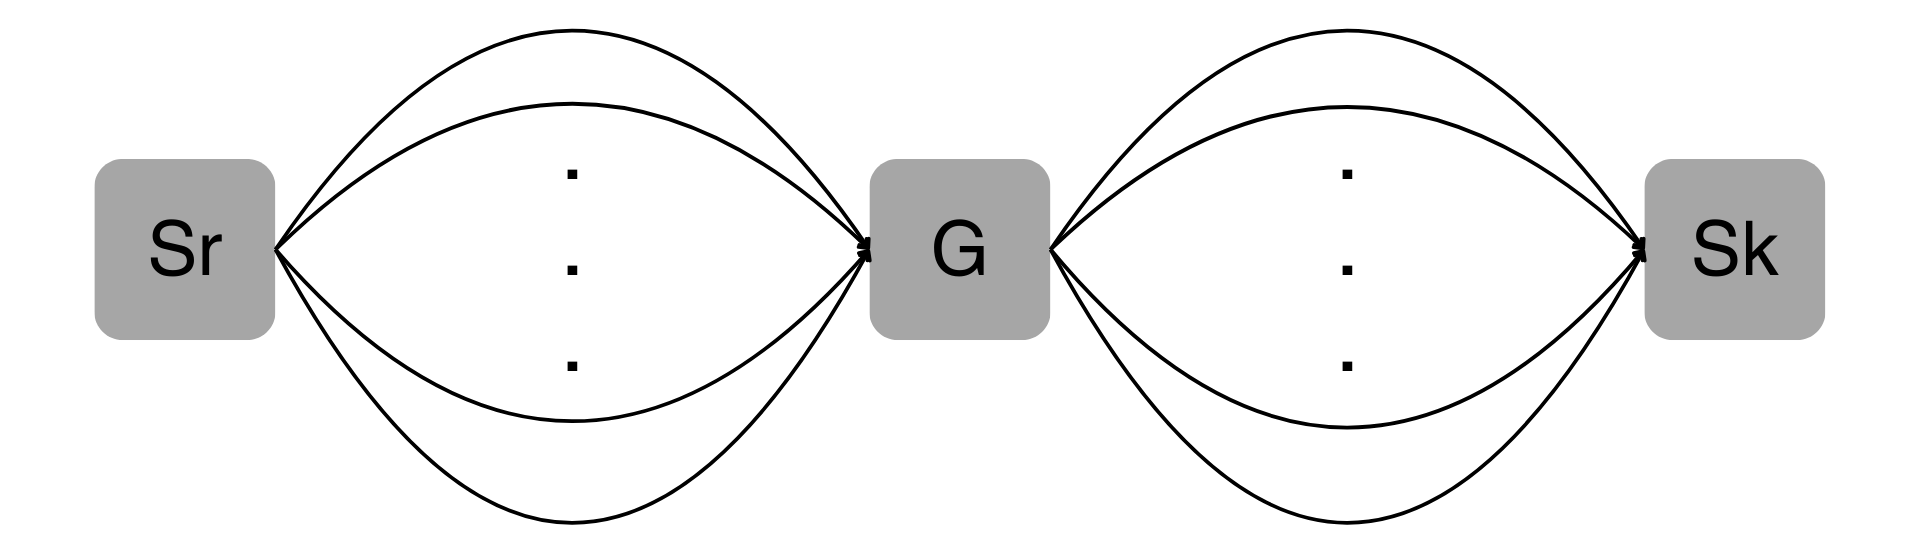
\includegraphics[width=1\textwidth]{DP100.png}
    \caption[{[Lib] Initia structure of a DP}]{This is the initial structure of a Dynamic Pipeline, self-made with Canva}
    \label{fig:DP100}
\end{figure}

\begin{figure}[H]
    \centering
    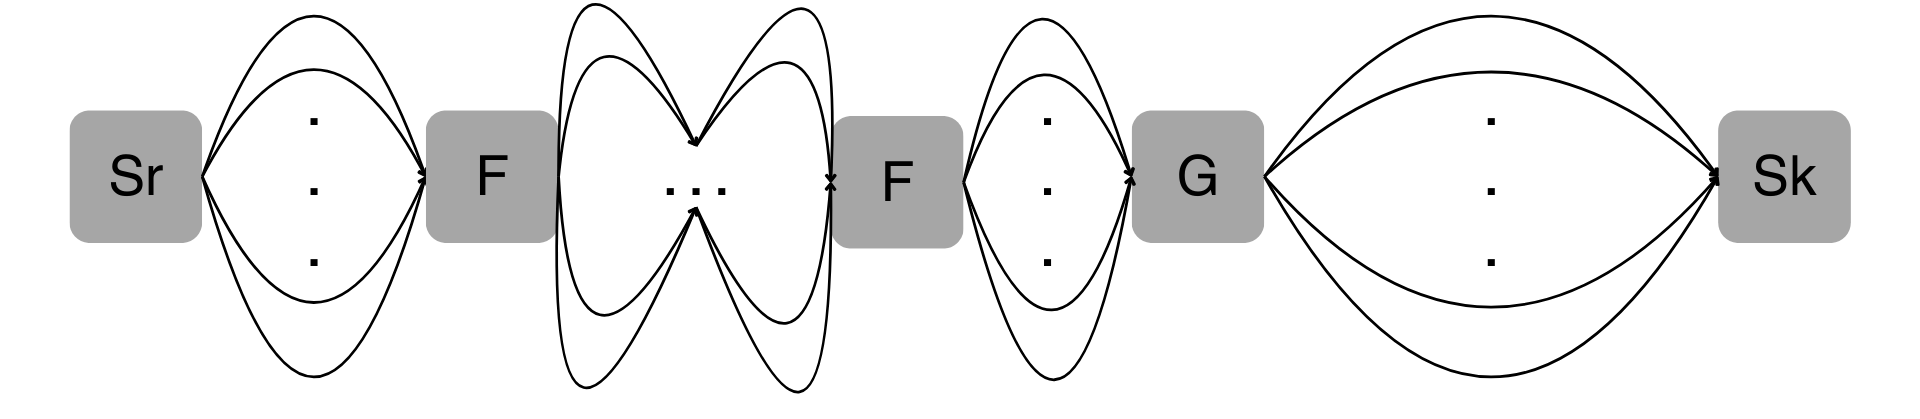
\includegraphics[width=1\textwidth]{DP101.png}
    \caption[{[Lib]} Posible structure of a DP]{This is a posible state of a Dynamic Pipeline, self-made with Canva}
    \label{fig:DP101}
\end{figure}

\subsection*{Source and Sink}
These two stages are the easiest to define and understand.
The Source and the Sink are responsible for introducing the input stream into the Pipeline and collecting the results and output them, respectively.
The Sr takes as input any form of data stream and is responsible for filling the different channels of the pipeline with data, which may already be processed and adapted by the stage itself.
At the end of the pipeline, the Sk is responsible for reading the different channels and returning the output to the outside.

\subsection*{Generator}
The Generator is more sophisticated and complex.
For each element it processes, it must decide whether to let it continue to the Sk and thus pass to the output or not.
In addition, it is responsible for deciding when to generate a Filter and add it to the pipeline.
For each element it reads, it can decide whether or not to generate a Filter, which is interposed between the last generated F (or the Sr if it is the first generated F) and itself.
It is also responsible for initializing the Filter by giving it a value for its parameter and its state.

\subsection*{Filter}
The last stage is the Filter.
It is the heart of the pipeline's computation and is responsible for processing and treating the data.
Each F has a state, which can be updated, and a parameter.
The execution of each filter is made up of a set of actors, which can be understood as the minimum unit of computation.
Each actor can consult the filter's parameter and state and update the latter.
It can also decide whether to pass on the data it processes and even generate new data to pass through the pipeline.
The actors are executed sequentially, one after the other, from the first to the last.

\section{Dynamic Pipeline Library}
Once we understand the basics of the Dynamic Pipeline paradigm, we can move on to review the library developed by Juan Pablo.
The first thing we can observe about the Haskell library is that it provides a set of types to work comfortably.
In general, there is one type for each concept of the dynamic pipeline (Sr, G, Sk, Channel, Actor, ...):

\begin{figure}[H]
    \begin{tabular}{c}
        \begin{lstlisting}
data Sink
data Generator (a :: Type), a (*$\sim$*) Channel
data Source (a :: Type), a (*$\sim$*) Channel
data FeedbackChannel (a :: Type), a (*$\sim$*) Channel
data Channel (a :: Type), a (*$\sim$*) (Type :<+> ... :<+> Eof)
data DynamicPipeline dpDef filtStat filterParam st, 
     dpDef (*$\sim$*) Source (Channel ..):=> 
                    Generator(Channel ..):=>Sink
data a :=> b, a & b (*$\sim$*) Stage
        \end{lstlisting}
    \end{tabular}
    \caption[{[Code]}Library data types]{These are some data types provided by the library}
    \label{fig:HC1}
\end{figure}

Based on these initial type definitions, we can see that the library provides us with the mecanism to define the DynamicPipeline type, which will determine the structure of our pipeline.
We can observe that it starts with an Sr that has a set of homogeneous type channels connected to a G, which is also connected to the end of the pipeline Sk through homogeneous type channels. \\

The library also introduces the concept of a Feedback Channel, which is a channel that allows feedback from the Generator (G) back into the pipeline.
This means that we can optionally add an additional stage with the sole task of feeding processed data back to the Source (Sr).
We will delve deeper into this topic later.

\subsection{Library combinators}
The library also provides a set of combinators (functions) for creating the different stages (Sr, G, Sk, and F).
The syntax of these functions can be quite complex, making them difficult to understand.
Since the goal of my work is not to fully comprehend the library and the underlying Haskell grammar, I will instead focus on explaining the concept of these functions and how to use them in a more straightforward manner.
This will enable anyone with a basic understanding of Haskell to implement their own Dynamic Pipeline for their specific problem.

\begin{figure}[H]
    \begin{tabular}{c}
        \begin{lstlisting}
withSource :: Stage (WithSource dpDef (DP st))
withGenerator :: Stage (WithGenerator dpDef filter (DP st))
withSink :: Stage (WithSink dpDef (DP st))
        \end{lstlisting}
    \end{tabular}
    \caption[{[Code]}Library combinators]{Some combinators provided by the library}
    \label{fig:HC2}
\end{figure}
Let's break down each combinator to understand how to use it to achieve the desired result.

\subsubsection*{Combinator withSource}

The withSource combinator is used to create a Source stage.
It takes a function as input (we will refere as fillChannels), which is responsible for filling the Source stage's output channels for any tipe of input.
This function receives the output channels of the Sr stage that are conected to G (or F) as arguments and should send data to these channels.

\begin{figure}[H]
    \begin{tabular}{c}
        \begin{lstlisting}
source :: Stage(   WriteChannel (*$t_1$*)
                -> WriteChannel (*$t_2$*)
                        .
                        .
                        .
                -> WriteChannel (*$t_n$*)
                -> DP st ()
                )
source = withSource @DPStructure . fillChannels

fillChannels ::WriteChannel (*$t_1$*)
            -> WriteChannel (*$t_2$*)
                    .
                    .
                    .
            -> WriteChannel (*$t_n$*)
            -> DP st ()
fillChannels (*$w_1$*) ... (*$w_n$*) = ...
        \end{lstlisting}
    \end{tabular}
    \caption[{[Code]}withSource combinator]{Function to get a Source stage using withSource combinator}
    \label{fig:HC3}
\end{figure}

Alright, this should be enough to create our Source stage.
We simply need to implement the fillChannels function to fill the different channels.
For this purpose, the library provides helper functions that simplify filling a channel from an input source (such as an array or a file).

\begin{figure}[H]
    \begin{tabular}{c}
        \begin{lstlisting}
--Feed a WriteChannel froma a Monadic Seed
unfoldM :: MonadIO m	 
        => m a	    --Monadic seed
        -> (a -> b) --Map input a to WriteChannel type b
        -> m Bool	--When stop unfolding
        -> WriteChannel b   --WriteChannel to feed	
        -> m () 

--Feed a WriteChannel from a file
unfoldFile :: MonadIO m	 
            => FilePath	          --FilePath to read from
            -> WriteChannel b     --WriteChannel to feed
            -> (ByteString -> b)  --Map ByteString to type b
            -> m ()

--Feed a WriteChannel from a foldable (like array)
unfoldT :: (MonadIO m, Foldable t) 
            => t a            --Foldable to unfold
            -> WriteChannel b --WriteChannel to feed
            -> (a -> b) --Map input a to WriteChannel type b
            -> m ()
        \end{lstlisting}
    \end{tabular}
    \caption[{[Code]}Fead channels]{Functions provided by library to fead channels}
    \label{fig:HC4}
\end{figure}

\subsubsection*{Combinator withSink}
Similar to withSource, the withSink combinator is used to create a Sink stage.
It takes a function as input (we will refere as readChannels), which is responsible for reading the Sink stage's input channels to output it.
This function receives the input channels coming from G as arguments and should output the results.

\begin{figure}[H]
    \begin{tabular}{c}
        \begin{lstlisting}
sink   :: Stage(   ReadChannel (*$t_1$*)
                -> ReadChannel (*$t_2$*)
                        .
                        .
                        .
                -> ReadChannel (*$t_n$*)
                -> DP st ()
                )
sink = withSink @DPStructure . readChannels

readChannels ::ReadChannel (*$t_1$*)
            -> ReadChannel (*$t_2$*)
                    .
                    .
                    .
            -> ReadChannel (*$t_n$*)
            -> DP st ()
readChannels (*$r_1$*) ... (*$r_n$*) = ...
        \end{lstlisting}
    \end{tabular}
    \caption[{[Code]}withSink]{Function to get a Sink stage using withSink combinator}
    \label{fig:HC5}
\end{figure}

With this steps, similar to withSource, should be enough to create our Sink stage.
We simply need to implement the readChannels function to output the results.
For this purpose, the library do not provide much help, we have just a function to read a channel and fill a generic output.

\begin{figure}[H]
    \begin{tabular}{c}
        \begin{lstlisting}
--Read a ReadChannel and fold it with a monadic function
foldM_ :: MonadIO m	 
        => ReadChannel a --ReadChannel to read
        -> (a -> m ())  --Computation to do with read element
        -> m ()
        \end{lstlisting}
    \end{tabular}
    \caption[{[Code]}Read channels]{Functions provided by library to read channels}
    \label{fig:HC6}
\end{figure}

\subsubsection*{Combinator withGenerator}
Finally, we have the withGenerator combinator, which is similar to the previous two but with some additional nuances.
As we recall, the G stage has both input and output channels, and it is also responsible for generating F stages.
Therefore, it must determine which of the read data should be passed to the output channels and what conditions must be met to generate an F stage.

The withGenerator combinator takes a function as input, which we will refer to as the genAction function.
This function is responsible for handling all the tasks mentioned above.

\begin{figure}[H]
    \begin{tabular}{c}
        \begin{lstlisting}
generator :: Stage(Filter DPExample filtStat filtPar st
                -> ReadChannel (*$t_1$*)
                        .
                        .
                        .
                -> ReadChannel (*$t_n$*)
                -> WriteChannel (*$t_1$*)
                        .
                        .
                        .
                -> WriteChannel (*$t_n$*)
                -> DP st ()
                )
generator = withGenerator @DPStructure . genAction

genAction ::   Filter DPExample filtStat filtPar st   
            -> ReadChannel (*$t_1$*)
                    .
                    .
                    .
            -> ReadChannel (*$t_n$*)
            -> WriteChannel (*$t_1$*)
                    .
                    .
                    .
            -> WriteChannel (*$t_n$*)
            -> DP st ()
genAction filter (*$r_1$*) ... (*$r_n$*) (*$w_1$*) ... (*$w_n$*) = ...
        \end{lstlisting}
    \end{tabular}
    \caption[{[Code]} withGenerator]{Function to get a Generator stage using withGenerator combinator}
    \label{fig:HC7}
\end{figure}

To create our G stage, we simply need to implement the genAction function.
The library provides helper functions that can simplify this task:

\begin{figure}[H]
    \begin{tabular}{c}
        \begin{lstlisting}
--Read a ReadChannel and fold it with a monadic function
unfoldF::UnFoldFilter dpDef readElem st filtStat filtPar l	
        -> DP st (HList l)

mkUnfoldFilter :: 
(readElem -> Bool)  --For each element determine if 
                    --interpose a new Filter
-> (readElem -> DP st ()) --For each element that the Filter 
                    --is consuming allow to do something 
                    --outside the filter with that element.
-> Filter dpDef filtStat filterParam st   --Filter Template
-> (readElem -> filtStat) --How to Initiate Internal
                             --Filter StateT (Memory)
-> ReadChannel readElem --Main ReadChannel to feed filter
-> HList l --Rest of the ReadChannels if there are needed
           --(HNil if it only contians 1)
-> UnFoldFilter dpDef readElem st filtStat filterParam l
        \end{lstlisting}
    \end{tabular}
    \caption[{[Code]} unfoldF and mkUnfoldFilter]{Functions unfolF and mkUnfoldFilter that help to implement genAction}
    \label{fig:HC8}
\end{figure}
By composing these two functions, we can generate our G stage.
The library also provides some variations of the mkUnfoldFilter function for easier use (see functions mkUnfoldFilter', mkUnfoldFilterForAll, mkUnfoldFilterForAll').
\subsection{Library smart constructors}
The next set of functions provided by the library to complete our Dynamic Pipeline implementation are Smart Constructors.
In Haskell, a smart constructor is a function that allows us to generate a result in a controlled manner and apply restrictions.
Using them ensures that we meet the necessary conditions and invariants for the correct operation of the pipeline.
\subsubsection*{mkFilter Smart Constructor}
The first smart constructor function provided by the library is mkFilter.
This function allows us to define a F stage with a single actor (logical unit).

\begin{figure}[H]
    \begin{tabular}{c}
        \begin{lstlisting}
filterTemp :: Filter dpDef filtStat filterParam st
filterTemp = mkFilter actor1

actor1 :: filterParam
        -> ReadChannel (*$t_1$*)
                .
                .
                .
        -> ReadChannel (*$t_n$*)
        -> WriteChannel (*$t_1$*)
                .
                .
                .
        -> WriteChannel (*$t_n$*)
        -> StateT filtStat (DP st) ()
actor_1 par (*$r_1$*) ... (*$r_n$*) (*$w_1$*) ... (*$w_n$*) = ...
        \end{lstlisting}
    \end{tabular}
    \caption[{[Code]} mkFilter and actors]{mkFilter smart constructor with definition of an actor}
    \label{fig:HC9}
\end{figure}

Similar to the previous functions, we only need to provide the implementation of the actor of F.
Within this function, we have to determine what to do with each element it processes and decide whether to update the state of F, which elements to pass to the next filters, ...
Here are some functions to perform most of the actions mentioned previously:

\begin{figure}[H]
    \begin{tabular}{c}
        \begin{lstlisting}
-- Push element a into WriteChannel
push :: MonadIO m 
        => a 
        -> WriteChannel a 
        -> m ()

-- Pull element Maybe a from ReadChannel
pull :: MonadIO m 
        => ReadChannel a 
        -> m (Maybe a)

-- Fetch the current value of the state within the monad
get :: Monad m 
    => StateT s m s

-- Sets the state within the monad to s
put :: Monad m 
    => s 
    -> StateT s m ()
        \end{lstlisting}
    \end{tabular}
    \caption[{[Code]}Building actors]{Some functions to implemet the actors}
    \label{fig:HC10}
\end{figure}

It should also be noted that filters can have more than one actor.
The library provides two functions for creating filters with N actors:

\begin{figure}[H]
    %\centering
    \begin{tabular}{c}
        \begin{lstlisting}
-- Add a new Actor to an already existing Filter.
(|>>>) :: Actor dpDef filtStat filterParam 
                (StateT filtStat (DP st))
        -> Filter dpDef filtStat filterParam st	
        -> Filter dpDef filtStat filterParam st

-- Given 2 Actors build a Filter.
(|>>) :: Actor dpDef filtStat filterParam 
                (StateT filtStat (DP st))
    -> Actor dpDef filtStat filterParam 
                (StateT filtStat (DP st))	
    -> Filter dpDef filtStat filterParam st       
        \end{lstlisting}
    \end{tabular}
    \caption[{[Code]} Building filters]{Function to create a filter with N actors}
    \label{fig:HC11}
\end{figure}

\subsubsection*{mkGenerator Smart Constructor}
This second smart constructor allows us to link our definition of G with our definition of F.
Simply passing our 2 previously defined functions as arguments to the function, we obtain a stage that encompasses our 2 definitions and combines them:
\begin{figure}[H]
    %\centering
    \begin{tabular}{c}
        \begin{lstlisting}
mkGenerator :: Stage (WithGenerator dpDef 
             (Filter dpDef filtStat filterParam st) (DP st))	
            -> Filter dpDef filtStat filterParam st	
            -> GeneratorStage dpDef filtStat filterParam st
            
generatorStage::GeneratorStage dpDef filtStat filterParam st
generatorStage = mkGenerator generator filterTemp
        \end{lstlisting}
    \end{tabular}
    \caption[{[Code]}mkGenerator ]{mkGenerator combinator}
    \label{fig:HC12}
\end{figure}

\subsubsection*{mkDP Smart Constructor}
This is the final combiner. It takes the three previously defined definitions (source, sink, generatorStage) and combines them to obtain our dynamic pipeline.
\begin{figure}[H]
    %\centering
    \begin{tabular}{c}
        \begin{lstlisting}
mkDP :: Stage (WithSource dpDef (DP st))	
    -> GeneratorStage dpDef filtStat filterParam st	
    -> Stage (WithSink dpDef (DP st))	
    -> DP st ()

DP' :: DP st ()
DP' = mkDP source generatorStage sink
        \end{lstlisting}
    \end{tabular}
    \caption[{[Code]} mkDP]{mkDP combinator}
    \label{fig:HC13}
\end{figure}
\subsection{Conclusions}
With all of this, we have all the elements to execute our Dynamic Pipeline.
The library give us a function that, given a pipeline, run it to final output result.
\begin{figure}[H]
    \begin{tabular}{c}
        \begin{lstlisting}
runDP :: DP st () 
        -> IO a
    
main :: IO ()
main = runDP DP'
        \end{lstlisting}
    \end{tabular}
    \caption[{[Code]} runDP]{runDP function for runing a DP}
    \label{fig:HC14}
\end{figure}

In this section, we have reviewed the entire library to extract the key concepts and tools necessary to implement the vast majority of Dynamic Pipelines.
We have observed how, using the functions provided by the library, it is only necessary to implement a few basic functions corresponding to the essential functionalities of the pipeline itself.
In this way, anyone with a Dynamic Pipeline algorithm can implement it with just some basic Haskell notions. \\

Here is a summary of the functions to implement for each pipeline:

\begin{figure}[H]
    %\centering
    \begin{tabular}{c}
        \begin{lstlisting}
-- Function defining what we put in each channel
fillChannels ::WriteChannel (*$t_1$*)
            -> WriteChannel (*$t_2$*)
                    .
                    .
                    .
            -> WriteChannel (*$t_n$*)
            -> DP st ()

-- Function defining what we do with the final data
readChannels ::ReadChannel (*$t_1$*)
            -> ReadChannel (*$t_2$*)
                    .
                    .
                    .
            -> ReadChannel (*$t_n$*)
            -> DP st ()


genAction ::   Filter DPExample filtStat filtPar st   
            -> ReadChannel (*$t_1$*)
                    .
                    .
                    .
            -> ReadChannel (*$t_n$*)
            -> WriteChannel (*$t_1$*)
                    .
                    .
                    .
            -> WriteChannel (*$t_n$*)
            -> DP st ()

-- Function defining an actor of a filter
actorN :: filterParam
        -> ReadChannel (*$t_1$*)
                .
                .
                .
        -> ReadChannel (*$t_n$*)
        -> WriteChannel (*$t_1$*)
                .
                .
                .
        -> WriteChannel (*$t_n$*)
        -> StateT filtStat (DP st) ()
        \end{lstlisting}
    \end{tabular}
    \caption[{[Code]}Functions summary]{Functions to implement for a DP}
    \label{fig:HC15}
\end{figure}

\section{Implementing the toy problem}
At this point, we have understood the two fundamental aspects: how a dynamic pipeline works and how to define and implement one.
In this section, we will walk through the entire process of defining and implementing a dynamic pipeline using a toy problem.
The goal is to present an example and obtain a template for future implementations of different problems.
\subsection{Algorithm Definition}
The task at hand is to implement a word counting algorithm using a dynamic pipeline.
The goal is to incrementally process a stream of characters, counting the occurrences of each word, and printing partial results whenever a period ('.') character is encountered.
This approach leverages the incremental nature of dynamic pipelines to provide real-time updates. \\

I will not delve deeply into the process of designing the algorithm itself, as the idea is to focus on the implementation.
Therefore, I will explain my proposed solution for the problem and carry out a small test run to understand the behavior.
To keep my design simple, it will only have one channel, and the filters will only have one actor.
This will minimize the complexity of understanding. Since we only have one channel, the data type that will flow will be tuples (Word, Int).
This will represent a specific word along with its count of how many times it appears.
It should be noted that since there is only one channel, the input data and the data generated by the filters themselves (solutions) will go on the same channel, so a rule will have to be created to differentiate them.

\subsubsection*{Source}
Alright, in our case, the Sr will need to obtain the words from the stream and feed the channel with tuples (Word, Int).
Since these are the input elements, we will initialize the tuple with (Word, 0).
This way, we can differentiate the input data from the solutions (since we know that the solutions will have at least a count of 1).

\begin{figure}[H]
    \centering
    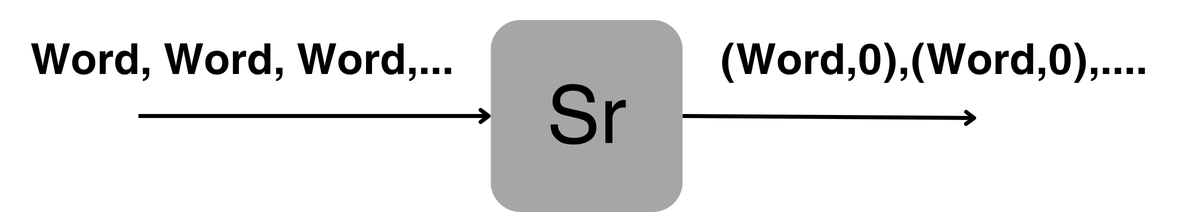
\includegraphics[width=1\textwidth]{DP102.png}
    \caption[{[Lib]} Source stage]{Grafic representation of the Source stage}
    \label{fig:DP102}
\end{figure}

\subsubsection*{Sink}
This stage is the simplest, as it only has to collect the results and display them.
The Sk will receive tuples (Word, Int) and should display them (to the console or a file, for example) in the desired format.

\begin{figure}[H]
    \centering
    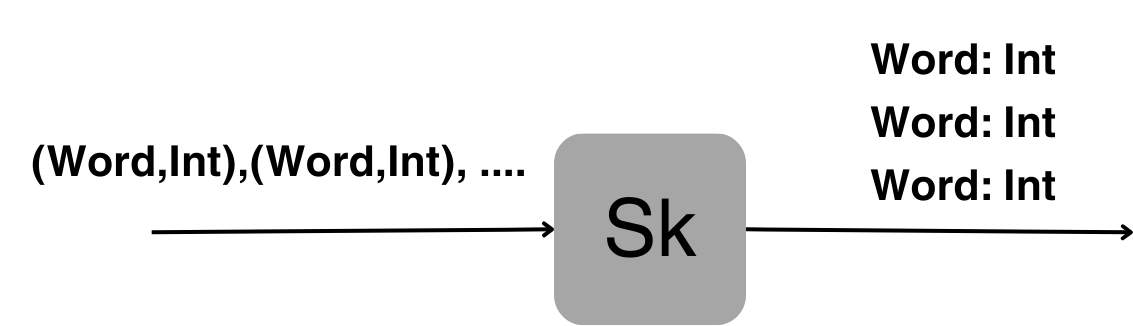
\includegraphics[width=1\textwidth]{DP103.png}
    \caption[{[Lib]} Sink stage]{Grafic representation of the Sink stage}
    \label{fig:DP103}
\end{figure}

\subsubsection*{Generator}
Now let's move on to the heart of the pipeline, the Generator.
This takes care of several tasks, so let's go through them one by one:

\begin{itemize}
    \item \textbf{Create Filters:} For each element it reads, it must decide whether or not to create a F.
    For our problem, the most sensible thing would be to have one filter for each unique word, so the G must ensure that it does not create two filters for the same word.
    To do this, we can take advantage of the fact that filters can also decide not to let words pass.
    We can leave the responsibility of not letting repeated words pass to the filters and have the G create an F for each word that reaches it, since this will be, in any case, the first appearance.

    \item \textbf{Initialize Filters:} The G must be responsible for initializing the state and parameter of the F.
    As mentioned previously, each F will handle a different word, so the most logical thing is to initialize the parameter with the word it handles (since it does not change).
    On the other hand, the state will have the appearance counter, so it can be updated with each new appearance.

    \item \textbf{Pass the elements:} It must decide which elements to pass on to the Sk to be displayed.
    With the rules we have created, we know that every tuple (Word, 0) is an input element that has not yet been processed, so we must discard it.
    On the other hand, if the counter is at least 1, we know that it comes from a filter, so it will be a result.
    Therefore, we will only pass non-initial elements, that is, those with a counter different from 0.
\end{itemize}

With all this defined, we have our G created and we can move on with the last stage.

\subsubsection*{Filter}
To finish, let's define the F.
At this point, we know that its parameter contains the word it handles and that its state contains the word count, so the logic that remains to be defined is quite simple.
The filter may receive words equal to its own, in which case it will have to update its counter by adding 1 and discarding the word, or different words, in which case it will simply let them pass.
With this logic, we can keep the counter updated at all times and meet the requirements on which the other stages are based (not letting repeated words pass).

The only thing left would be to introduce the incremental component mentioned at the beginning of the section.
'.' could arrive, which represent a signal to indicate to the F's that they should pass a partial response.
Therefore, before starting the logic, they will have to check if the input is a '.' , so they will have to take the state and join it with the parameter in a tuple with the form (parameter, tuple) followed by the point so that the rest of the filters do the same. In case it is not a '.', the same logic mentioned above will be done.

\subsection{Algorithm Simulation}
With all the stages defined, we can now simulate the algorithm for better understanding. \\

We start the simulation, this is our initial state of the pipeline.
As input we have a string of words 'Dog', 'Cat', 'Dog' ended by a '.'.

\begin{figure}[H]
    \centering
    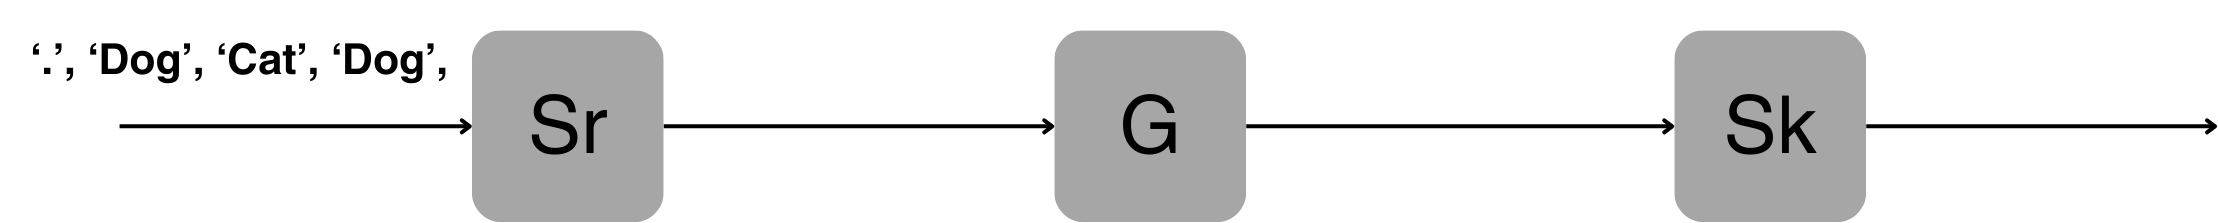
\includegraphics[width=1\textwidth]{DP104.png}
    \caption[{[Lib]} Counting words inital state]{Initial state of the Dynamic Pipeline with the input prepared}
    \label{fig:DP104}
\end{figure}

The first word, 'Dog', will go through the Sr and turn it into a tuple (Dog, 0).
This reaches the generator and generates the first filter, since it is an initial data (counter to 0).
The Sr continues to process the input while following the process.

\begin{figure}[H]
    \centering
    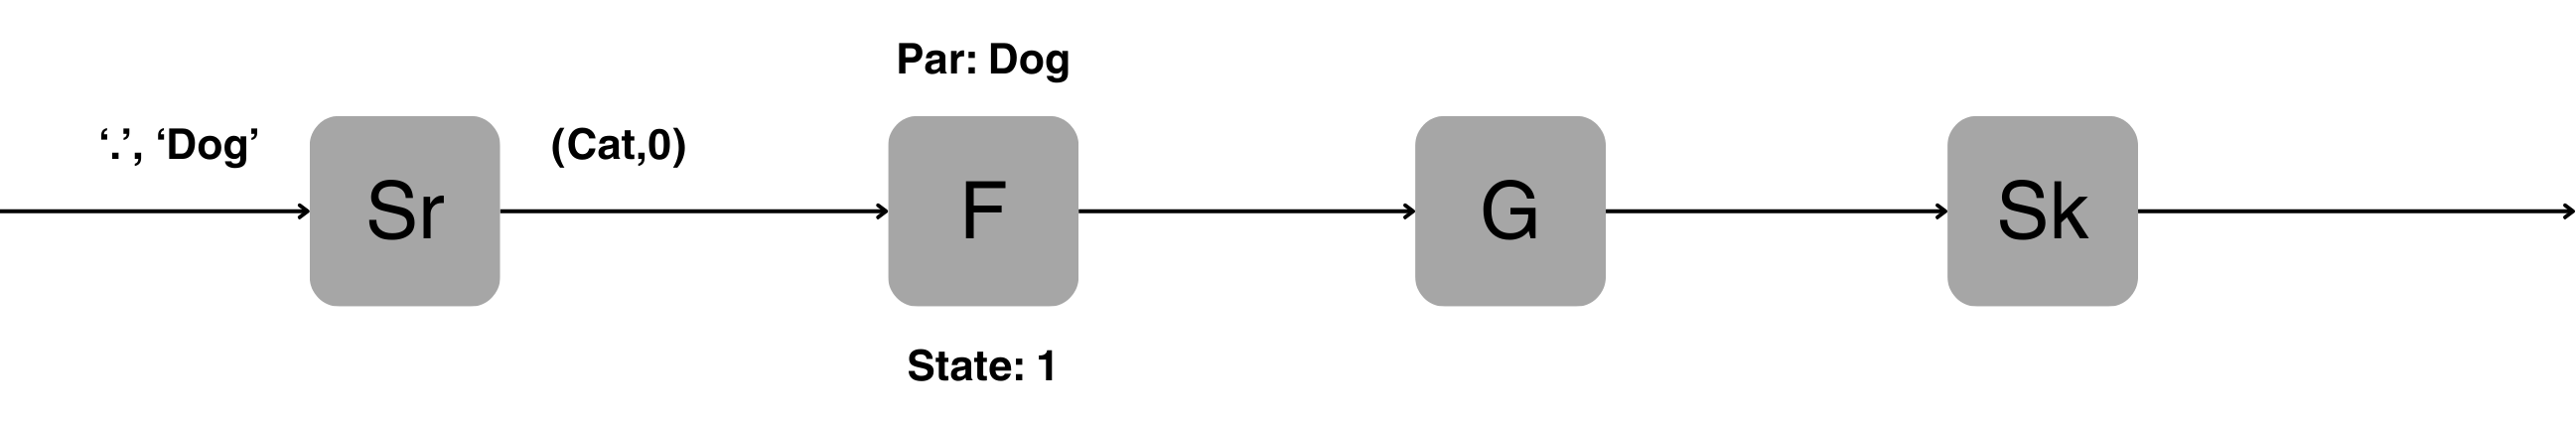
\includegraphics[width=1\textwidth]{DP105.png}
    \caption[{[Lib]} Counting words state 1]{State of Dynamic Pipeline after consuming some words}
    \label{fig:DP105}
\end{figure}

If we continue executing until just after the Sr processes the '.', this is the state of our pipeline:

\begin{figure}[H]
    \centering
    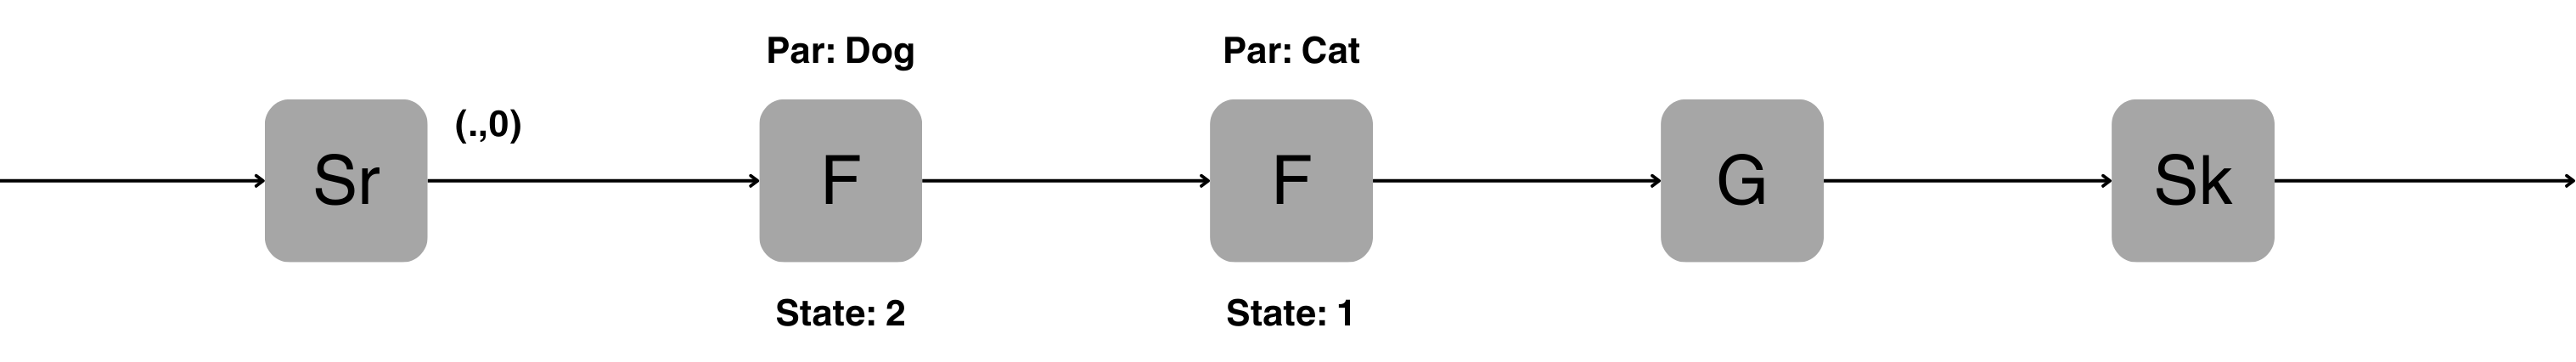
\includegraphics[width=1\textwidth]{DP106.png}
    \caption[{[Lib]} Counting words state 2]{State of Dynamic Pipeline before the '.' is processed by filters}
    \label{fig:DP106}
\end{figure}

When the '.' starts to be processed by F's, they with start to throw partial results.
This is the view of the pipeline before the second F starts to process the '.'.

\begin{figure}[H]
    \centering
    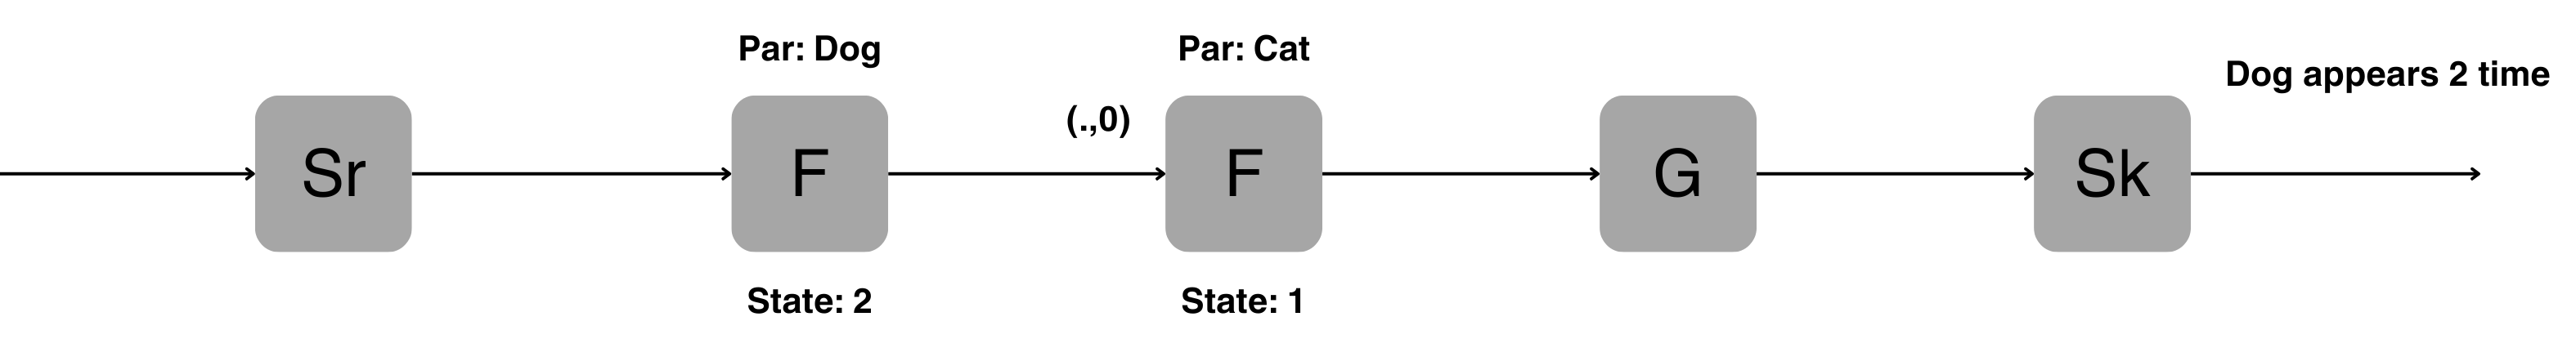
\includegraphics[width=1\textwidth]{DP107.png}
    \caption[{[Lib]} Counting words state 3]{State of Dynamic Pipeline before the the second filter processes the '.'}
    \label{fig:DP107}
\end{figure}

And this is the final state after the whole execution:

\begin{figure}[H]
    \centering
    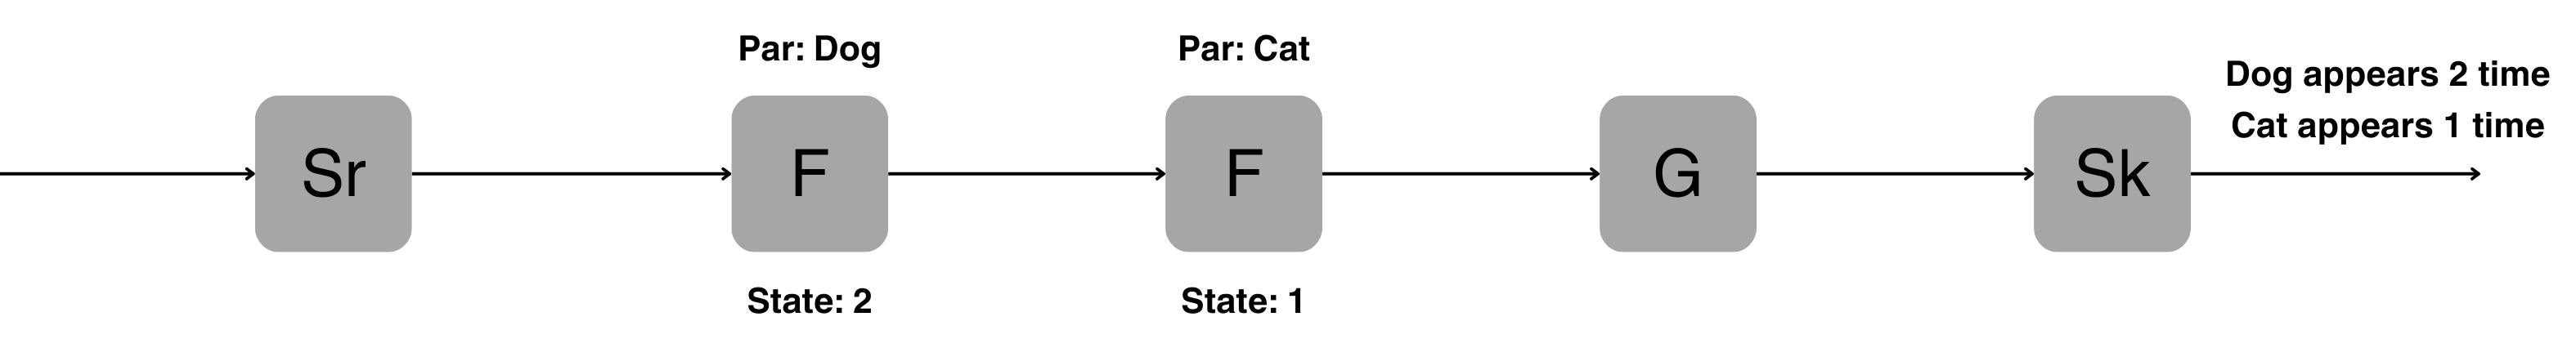
\includegraphics[width=1\textwidth]{DP108.png}
    \caption[{[Lib]} Counting words final state]{Final state of the Dynamic Pipeline}
    \label{fig:DP108}
\end{figure}

\subsection{Algorithm Implementation}
Now we have all the components necessary to use the library in a real case: We understand how a Dynamic Pipeline works, we know how to implement it using the Haskell library and we have defined an algorithm for a specific problem. Now we just have to apply everything.
\subsubsection*{Type definition}
Let's start by defining our Dynamic Pipeline structure in Haskell:

\begin{figure}[H]
    %\centering
    \begin{tabular}{c}
        \begin{lstlisting}
type Word = String
type Pair = (Word,Int)
type filtStat = Int
type filtPar = Pair
type DPExample = Source (Channel (Pair :<+> Eof)) 
                :=> Generator (Channel (Pair :<+> Eof)) 
                :=> Sink
        \end{lstlisting}
    \end{tabular}
    \caption[{[Code]} Implementation 1]{Type definition of the Dynamic Pipeline}
    \label{fig:HC16}
\end{figure}

I've also defined some additional types for the tuples and for the state and parameters of the F filter, for simplicity.

\subsubsection*{Source}
As we determined earlier, to define the source we only have to implement 1 function (which we have called fillChannels)

\begin{figure}[H]
    \begin{tabular}{c}
        \begin{lstlisting}
input :: [Word]
input = ["Dog","Cat","Dog","."]

source' :: Stage (WriteChannel Pair -> DP s ())
source' = withSource @DPExample fillChannels

fillChannels :: WriteChannel Pair
             -> DP st ()
fillChannels wp = unfoldT input wp (*\$*) \w -> (w,0)
        \end{lstlisting}
    \end{tabular}
    \caption[{[Code]} Implementation 2]{Implementation of fillChannels function}
    \label{fig:HC17}
\end{figure}

We can observe how the fillChannels function uses the unfoldT function provided by the library to read an array and pass it through a write channel.
We also use an anonymous function to transform the words into tuples.

\subsubsection*{Sink}
For this stage, we need to implement the readChannels function:

\begin{figure}[H]
    %\centering
    \begin{tabular}{c}
        \begin{lstlisting}
sink' :: Stage (ReadChannel Pair -> DP s ())
sink' = withSink @DPExample readChannels

readChannels ::ReadChannel Pair -> DP st ()
readChannels rp = foldM_ rp printResults

printResults :: Pair -> DP st ()
printResults (".",_) = print "**********************"
printResults (w,n) = print $ w ++ " " ++ show n

        \end{lstlisting}
    \end{tabular}
    \caption[{[Code]} Implementation 3]{Implementation of readChannels function}
    \label{fig:HC18}
\end{figure}

In this case, we use the unique function provided by the library: foldM function.
It reads a channel and do a function, in this case, print the results.

\subsubsection*{Filter}
For the F we need to implement all the actors.
As we have only one actor, we will only implement one function.

\begin{figure}[H]
    %\centering
    \begin{tabular}{c}
        \begin{lstlisting}
filterTemp :: Filter DPExample filtStat filtPar s 
filterTemp = mkFilter actor1

actor1 :: filtPar
        -> ReadChannel Pair
        -> WriteChannel Pair
        -> StateT filtStat (DP s) ()
actor1 (par,_) rp wp =
  foldM_ rp (*\$*) \(inp,y) -> 
    if inp == "." 
    then get >>= \x -> push (par,x) wp >> push (".",0) wp
    else    if inp == par
            then modify (+1)
            else push (inp,y) wp
        \end{lstlisting}
    \end{tabular}
    \caption[{[Code]} Implementation 4]{Implementation of actor}
    \label{fig:HC19}
\end{figure}

As we defined before, it treats each element with the foldM function following the chain of if's: first if it's a period, where it would pass the result and the period.
Otherwise, it would update the state with the modify function or simply let the word pass through.

\subsubsection*{Generator}
Finally, we have to implement the G stage:

\begin{figure}[H]
    %\centering
    \begin{tabular}{c}
        \begin{lstlisting}
generator' :: GeneratorStage DPExample filtStat filtPar s
generator' = let gen = withGenerator @DPExample genAction
            in  mkGenerator gen filterTemp

genAction :: Filter DPExample filtStat filtPar s
          -> ReadChannel Pair
          -> WriteChannel Pair
          -> DP s ()
genAction filter rp wp =
  let unfoldFilter = 
  mkUnfoldFilter create (moveOn wp) filter iniFilter rp HNil
  in void $ unfoldF unfoldFilter

create :: Pair-> Bool
create (".",_) = False
create (_,0) = True
create _ = False

moveOn :: WriteChannel Pair -> Pair -> DP s ()
moveOn c (".",_) = push (".",0) c
moveOn _ (_,0) = return ()
moveOn c a = push a c

iniFilter :: Pair -> filtStat
iniFilter _ = 1
        \end{lstlisting}
    \end{tabular}
    \caption[{[Code]} Implementation 5]{Implementation of generator}
    \label{fig:HC20}
\end{figure}

This stage involves defining the most functions, although the mkUnfoldFilter constructor aids significantly in implementation.
The three generator functionalities must be implemented: determining under which conditions to generate a filter, initializing a filter, and deciding which elements to pass through.
To achieve this, three functions have been defined: create, iniFilter, and moveOn, which handle the aforementioned functionalities, respectively.
The \textit{create} function takes an element of the input channel type and returns a boolean value indicating whether or not to generate a filter. \\
Similarly, the \textit{iniFilter} function takes an element of the input channel type and returns an element of the filter state type. \\
Finally, the \textit{moveOn} function receives both the write channel and an element of the channel type and decides whether to push the element or do nothing (effectively discarding the element). 

\subsection{Conclusions}
In this section, we have seen the entire process for implementing a simple problem like counting words.
To test its effectiveness, some tests have been carried out. This is a tested input:

\begin{center}
input = ["dog", "cat",".","dog","dog","dog",".","bird","cat","."]
\end{center}
And this has been the result obtained:

\begin{center}
"dog 1" \\
"cat 1" \\
"**********************" \\
"dog 4" \\
"cat 1" \\
"**********************" \\
"dog 4" \\
"cat 2" \\
"bird 1" \\
"**********************" \\
\end{center}

Therefore, we can conclude that the implementation has been developed successfully
\section{Improving the library}
After working with the library, I have been able to identify different shortcomings and lack of functionalities for a more diverse and easier use of the library.
In this section, I will detail and comment on different improvements that I have added to the library.

\subsection{New features}
\subsubsection*{unfoldFilebyChars}

When I was working with the library, the first thing I missed was having more tools to work with the input.
The library has the functions unfoldM, unfoldFile, and unfoldT to handle general monadic inputs, files, and lists, respectively.
The problem is that the unfoldFile function only reads files line by line, since that's how it was useful for Juan Pablo's problem.
That's why I decided to create this function to be able to read character by character for letters of the alphabet.
In this way, the channel is fed with characters and it can be, for example, the F or the G that are responsible for finding the desired format.

\begin{figure}[H]
    %\centering
    \begin{tabular}{c}
        \begin{lstlisting}
unfoldFilebyChars :: FilePath 
                    -> WriteChannel a 
                    -> (ByteString -> a) 
                    -> DP s ()
unfoldFilebyChars file writeChannel fn =
  liftIO $ R.withFile file ReadMode $ \h -> 
        unfoldM (hGetchar h) fn (H.hIsEOF h) writeChannel

hGetchar :: Handle -> IO ByteString
hGetchar h = do
    c <- hGet h 1
    if c == "" || c == "." || "a" <= c && c <= "z" 
    then return c 
    else hGetchar h
        \end{lstlisting}
    \end{tabular}
    \caption[{[Code]} unfoldFilebyChars definition]{unfoldFilebyChars function}
    \label{fig:HC21}
\end{figure}

An example usage of the function is as follows:

\begin{figure}[H]
    %\centering
    \begin{tabular}{c}
        \begin{lstlisting}
-- Write Channel (wc) Type = String
unfoldFilebyChars "example.txt" wc decodeUtf8	
        \end{lstlisting}
    \end{tabular}
    \caption[{[Code]} unfoldFilebyChars example]{unfoldFilebyChars function usage}
    \label{fig:HC21b}
\end{figure}

\subsubsection*{unfoldFilebyWords}
Similar to the previous function, this function feeds a channel from a file by reading the words.
It separates the input by the blank space character ' ' similar to the getContents function in Haskell. \\

This improvement is quite significant, offering considerably more flexibility than the existing function.
The ability to retrieve content item by item rather than the entire row facilitates simpler input processing.
\begin{figure}[H]
    %\centering
    \begin{tabular}{c}
        \begin{lstlisting}
unfoldFilebyWords :: FilePath 
            -> WriteChannel a --Write Channel to feed
            -> (ByteString -> a) --Map ByteString to type a
            -> DP s ()
unfoldFilebyWords file writeChannel fn = 
  liftIO $ R.withFile file ReadMode $ \h -> 
        unfoldM (hGetWord h) fn (H.hIsEOF h) writeChannel

hGetWord :: Handle 
        -> IO ByteString
hGetWord h = hGetWordRec h B.empty

hGetWordRec :: Handle 
            -> ByteString 
            -> IO ByteString
hGetWordRec h r = do
    c <- B.hGet h 1
    if c == "" || c == " " || c == "\n" then return r
    else do
        cs <- hGetWordRec h (B.append r c)
        return cs
        \end{lstlisting}
    \end{tabular}
    \caption[{[Code]} unfoldFilebyWords definition]{unfoldFilebyWords function}
    \label{fig:HC22}
\end{figure}

An example usage of the function is as follows:

\begin{figure}[H]
    %\centering
    \begin{tabular}{c}
        \begin{lstlisting}
-- Write Channel (wc) Type = String
unfoldFilebyWords "example.txt" wc decodeUtf8	
        \end{lstlisting}
    \end{tabular}
    \caption[{[Code]} unfoldFilebyWords example]{unfoldFilebyWords function usage}
    \label{fig:HC22b}
\end{figure}

\subsubsection*{pushState}
While not essential for the library's core functionality, this function aims to streamline the implementation process.
Often, retrieving and passing the filter state through a channel is required.
This function simplifies this task, enhancing ease of use.
Additionally, an optional function 'f' can be provided to convert the filter state type to the channel type.

\begin{figure}[H]
    %\centering
    \begin{tabular}{c}
        \begin{lstlisting}
pushState :: WriteChannel a --Write Channel to feed
            -> (b -> a) --Map state type to channel type
            -> StateT b (DP s) ()
pushState wp f = get >>= flip push wp . f
        \end{lstlisting}
    \end{tabular}
    \caption[{[Code]} pushState definition]{pushState function}
    \label{fig:HC23}
\end{figure}
An example usage of the function is as follows:

\begin{figure}[H]
    %\centering
    \begin{tabular}{c}
        \begin{lstlisting}
-- filtStat Type = Int
-- Write Channel (wc) Type = String
pushState wc show
        \end{lstlisting}
    \end{tabular}
    \caption[{[Code]} pushState example]{pushState function usage}
    \label{fig:HC23b}
\end{figure}

\subsubsection*{foldFile}
Another major problem I encountered was that the library also had almost no functions for handling output in a simple way.
The library has the foldM function, which is a very generic function for consuming a channel.
That's why I decided to add this function, which consumes a channel and writes it to an output file.
At the beginning of writing, the file is created if it does not exist, or the file is cleaned if it already existed. \\

This new functionality is highly desirable, especially when dealing with large inputs or performing analyses.
It allows us to gather all results in a convenient format, enabling more efficient processing and reading.

\begin{figure}[H]
    %\centering
    \begin{tabular}{c}
        \begin{lstlisting}
foldFile:: MonadIO m 
        => FilePath     --Path of file 
        -> (a -> Text)  -- Map WriteChannel type a to Text
        -> ReadChannel a --ReadChannel to read
        -> m ()
foldFile file f rc = do
  writeFileText file T.empty
  foldM_ rc (R.appendFileText file . f)
        \end{lstlisting}
    \end{tabular}
    \caption[{[Code]} foldFile definition]{foldFile function}
    \label{fig:HC24}
\end{figure}

An example usage of the function is as follows:

\begin{figure}[H]
    %\centering
    \begin{tabular}{c}
        \begin{lstlisting}
-- Read Channel (rc) Type = String
foldFile "example.txt" toText rc	
        \end{lstlisting}
    \end{tabular}
    \caption[{[Code]} foldFile example]{foldFile function usage}
    \label{fig:HC24b}
\end{figure}

\subsection{Updating the library to a newer version of GHC}
In this section, we will update the library to be compatible with newer versions of GHC, the Haskell compiler.
Currently, the library supports GHC version 8.10.3 and will be updated to support version 9.0.2.
This specific version was chosen as it's the latest supported by all libraries utilized by Dynamic Pipeline.
Particularly, the HList library introduces compatibility issues with newer GHC versions.
Updating the libraries would be necessary to leverage newer compiler versions.\\

The library consists of four source files: Flow.hs, Stage.hs, Channel.hs, and DynamicPipeline.hs.
DynamicPipeline is the main file and encompasses the other three, hence the need to update all of them.\\

This is the first error encountered when trying to compile DynamicPipeline.hs with the new GHC version:

\begin{figure}[H]
    %\centering
    \begin{tabular}{c}
        \begin{lstlisting}[escapeinside={(*}{*)}, language=bash]
DynamicPipeline/Stage.hs:515:9: (*\textcolor{red}{error:}*)
    Couldnt match type: DP st0 a
        with: forall (st :: k). DP st a
    Expected: (forall (st :: k). DP st a) -> IO a
        Actual: DP st0 a -> IO a
    In the expression: runStage
    In an equation for 'runDP': runDP = runStage
    Relevant bindings include
        runDP :: (forall (st :: k). DP st a) -> IO a
            (bound at DynamicPipeline/Stage.hs:515:1)
    (*\textcolor{blue}{|}*)
(*\textcolor{blue}{515}*)  (*\textcolor{blue}{|}*) runDP = (*\textcolor{red}{runStage}*)
    (*\textcolor{blue}{|}*)
        \end{lstlisting}
    \end{tabular}
    \caption[{[Lib] First console output} unfoldFilebyChars definition]{Console output after compiling DynamicPipeline.hs with GHC 9.0.2}
    \label{fig:HC25}
\end{figure}

And here is the code for the function that generates the error:

\begin{figure}[H]
    %\centering
    \begin{tabular}{c}
        \begin{lstlisting}
runDP :: (forall st. DP st a) -> IO a
runDP = runStage
        \end{lstlisting}
    \end{tabular}
    \caption[{[Code]} runDP error]{Piece of code generating the error}
    \label{fig:HC26}
\end{figure}
What we can gather from this error is that there's a type inference issue with the runDP function in the Stage.hs file.
Based on the observation, it seems that newer GHC versions are stricter with polymorphic types.
Delving into the GHC documentation, the first relevant information we find is that the initial GHC 9 release (9.0.1) introduced the following feature: \cite*[][Point 2.1.2.1]{} \\

\textit{"Record field selectors are now given type signatures that preserve the user-written order of quantified type variables.
Moreover, field selector type signatures no longer make inferred type variables available for explicit type application."}  \\

If we apply the new restrictions detailed in the release notes, our code would now look like this:

\begin{figure}[H]
    %\centering
    \begin{tabular}{c}
        \begin{lstlisting}
runDP :: forall {k} (st :: k) a. DP st a -> IO a
runDP = runStage
        \end{lstlisting}
    \end{tabular}
    \caption[{[Code]} New runDP definition]{New version of the code}
    \label{fig:HC27}
\end{figure}

As we can see now, we need to explicitly state that the type of st is any.
With this change, the compilation error no longer appears, so this part is now resolved.
However, when compiling again, there are still some errors to address.
There is a large output in the console, and here is some of the relevant information:

\begin{figure}[H]
    %\centering
    \begin{tabular}{c}
        \begin{lstlisting}[escapeinside={(*}{*)}, language=bash]
            .
            .
            .
DynamicPipeline/Stage.hs:408:29: (*\textcolor{red}{error:}*)
Couldnt match type 'b0'
    with MonadState filtStat monadicAction =>
    Stage (WithFilter dpDef filterParam monadicAction)
Expected: 
    Actor dpDef filtStat filterParam monadicAction
    -> b0
Actual: 
    Actor dpDef filtStat filterParam monadicAction
    -> MonadState filtStat monadicAction =>
    Stage (WithFilter dpDef filterParam monadicAction)
            .
            .
            .
    (*\textcolor{blue}{|}*)
(*\textcolor{blue}{408}*)  (*\textcolor{blue}{|}*) runActor = hUncurry . run . (*\textcolor{red}{unActor}*)
    (*\textcolor{blue}{|}*)
        \end{lstlisting}
    \end{tabular}
    \caption[{[Lib] Second console output}]{Second console output after compiling DynamicPipeline.hs with GHC 9.0.2}
    \label{fig:HC28}
\end{figure}

Similar to the previous error, here we also have a type inference problem.
Once again, the GHC update has made it stricter, causing us to have to modify the code to fix it.

If we see, the funcion unActor is the problem, so here is the code of the definition:

\begin{figure}[H]
    %\centering
    \begin{tabular}{c}
        \begin{lstlisting}
newtype Actor dpDef filtStat 
                filterParam monadicAction =
  Actor {unActor :: 
    MonadState filtStat monadicAction => 
  Stage (WithFilter dpDefinition filterParam monadicAction)}
        \end{lstlisting}
    \end{tabular}
    \caption[{[Code]} unActor error]{Piece of code generating the error}
    \label{fig:HC29}
\end{figure}

Starting with GHC version 9.0.1, it was added that new type definitions had to be explicit, so the way we have it here can no longer be used.
Therefore, we must leave the code like this:
\begin{figure}[H]
    %\centering
    \begin{tabular}{c}
        \begin{lstlisting}
newtype Actor dpDef filtStat 
                filterParam monadicAction =
Actor {unActor ::
  Stage (WithFilter dpDef filterParam monadicAction)}
        \end{lstlisting}
    \end{tabular}
    \caption[{[Code]} New unActor]{New version of the code}
    \label{fig:HC30}
\end{figure}
With these changes, we have now been able to compile the library with GHC 9.0.2.

\section{Chapter summary}
In this section, we have been able to improve the Haskell Dynamic Pipeline library.
We have added new features to make it easier to implement new algorithms, and we have also updated the library to support GHC 9.0.2.
With these advances, I aim to ensure that the library remains usable and does not become outdated.
At the end of the work \ref{experiments}, an experimental test will be carried out to verify if an improvement in the performance of the library has also been obtained.

